\documentclass{article}
\usepackage{tikz}
\usetikzlibrary{positioning}

\begin{document}

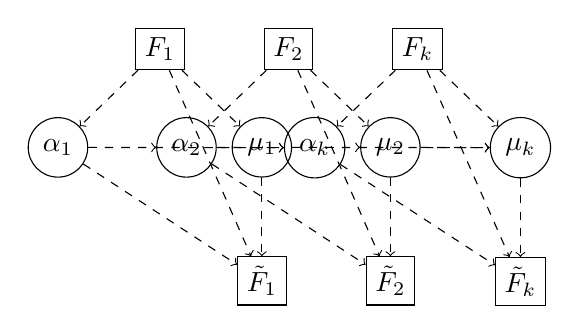
\begin{tikzpicture}[node distance=1cm, auto]
    % Define nodes
    \node [draw, rectangle] (F1) {$F_{1}$};
    \node [draw, rectangle, right=of F1] (F2) {$F_{2}$};
    \node [draw, rectangle, right=of F2] (Fk) {$F_{k}$};

    \node [draw, circle, below left=of F1] (alpha1) {$\alpha_{1}$};
    \node [draw, circle, below right=of F1] (mu1) {$\mu_{1}$};
    \node [draw, circle, below left=of F2] (alpha2) {$\alpha_{2}$};
    \node [draw, circle, below right=of F2] (mu2) {$\mu_{2}$};
    \node [draw, circle, below left=of Fk] (alphak) {$\alpha_{k}$};
    \node [draw, circle, below right=of Fk] (muk) {$\mu_{k}$};

    \node [draw, rectangle, below=of mu1] (Ftilde1) {$\tilde{F}_{1}$};
    \node [draw, rectangle, below=of mu2] (Ftilde2) {$\tilde{F}_{2}$};
    \node [draw, rectangle, below=of muk] (Ftildek) {$\tilde{F}_{k}$};

    % Draw edges
    \draw[->, dashed] (F1) -- (alpha1);
    \draw[->, dashed] (F1) -- (mu1);
    \draw[->, dashed] (F2) -- (alpha2);
    \draw[->, dashed] (F2) -- (mu2);
    \draw[->, dashed] (Fk) -- (alphak);
    \draw[->, dashed] (Fk) -- (muk);

    \draw[->, dashed] (alpha1) -- (Ftilde1);
    \draw[->, dashed] (alpha2) -- (Ftilde2);
    \draw[->, dashed] (alphak) -- (Ftildek);

    \draw[->, dashed] (mu1) -- (Ftilde1);
    \draw[->, dashed] (mu2) -- (Ftilde2);
    \draw[->, dashed] (muk) -- (Ftildek);

    \draw[->, dashed] (alpha1) -- (alpha2);
    \draw[->, dashed] (alpha1) -- (alphak);
    \draw[->, dashed] (alpha2) -- (alphak);

    \draw[->, dashed] (mu1) -- (mu2);
    \draw[->, dashed] (mu1) -- (muk);
    \draw[->, dashed] (mu2) -- (muk);

    \draw[->, dashed] (F1) -- (Ftilde1);
    \draw[->, dashed] (F2) -- (Ftilde2);
    \draw[->, dashed] (Fk) -- (Ftildek);
\end{tikzpicture}

\end{document}